\documentclass[spanish,a4paper,11pt]{article}
\usepackage[spanish]{babel}
\usepackage[utf8]{inputenc}
\usepackage{graphicx}
\footskip=27pt
\hoffset=0pt
\paperwidth=597pt
\begin{document}
\title{Informacion sobre numerp Pi}
\author{Andrés palenzuela \\
         técnicas experimentales~\footnote{universidad de la laguna}}
\date{10 de abril de 2014}
\maketitle
\begin{abstract}
Pi es la relación entre la longitud de una circunferencia y su diámetro, 
en geometría euclidiana. Es un número irracional y una de las constantes 
matemáticas más importantes. Se emplea frecuentemente en matemáticas, 
física e ingeniería.
\end{abstract}
\section{Historia del cálculo de Pi}
Nos encontramos con el número pi cuando dividimos la longitud de una circunferencia entre 
su diámetro. Podemos hallar una aproximación con cualquier objeto redondo como, por ejemplo, 
un bote de conservas.
\begin{itemize}
\item En Mesopotamia, los babilonios utilizaban el valor 3'125 según puede leerse en 
la Tablilla de Susa.
\item En China se hicieron esfuerzos para calcular su valor, Liu Hui utiliza polígonos 
de hasta 3072 lados para conseguir el valor de 3'14159. 
\end{itemize}
\section{Definiciones}
Euclides fue el primero en demostrar que la relación entre una circunferencia y su 
diámetro es una cantidad constante.No obstante, existen diversas definiciones del número Pi, 
pero las más común es la relacion entre la longitud de la circunferencia y su diametro, el 
área de un circulo unitario (de radio unidad de plano de euclídeo), entre otros.
bigskip
\subsection{Numero irracional y trascendente}
Se trata de un número irracional, lo que significa que no puede expresarse como fracción 
de dos números enteros, como demostró Johann Heinrich Lambert en 1761. También es un número 
trascendente, es decir, que no es la raíz de ningún polinomio de coeficientes enteros. En el 
siglo XIX el matemático alemán Ferdinand Lindemann demostró este hecho.\par
También se sabe que Pi tampoco es un número de Liouville, es decir, no sólo es trascendental 
sino que no puede ser aproximado por una secuencia de racionales "rápidamente convergente".
\subsection{Las primeras cincuenta cifras del numero Pi}
A pesar de tratarse de un número irracional continúa siendo averiguada la máxima cantidad 
posible de decimales.\par
En ciencia e ingeniería, esta constante puede emplearse, la mayoría de las veces, con una 
precisión de sólo una docena de decimales. Con cincuenta decimales se podría describir con 
precisión la curvatura del Universo con un error más pequeño que el tamaño de un 
protón\footnote{es una partícula subatómica con una carga eléctrica elemental positiva 1 }.

\begin{figure}[!th]
\begin{center}
\includegraphics[width=0.25\textwidth]{images/figura2.eps}
\caption{Número PI}
\label{num_pi}
\end{center}
\end{figure}

\begin{table}[!ht]
\begin{tabular}{|l|c|c|}
\hline
Nombre & Año & Aproximación\\ \hline
Papiro de Almes & 1650 a.C. & 3.16\\ \hline
Bandhayana & 500 a.C. & 3.09\\ \hline
Liu Hui & 260 d.C. & 3.1416\\ \hline
\end{tabular}
\cite{educacion}
\caption{Aproximaciones en la historia}
\label{tabla}
\end{table}

\end{document}
 
